\documentclass[a4paper,
12pt,footsepline,oneside,			
plainfootsepline,listof=totoc,headinclude,
footinclude]{scrreprt}
\usepackage{graphicx}
\usepackage[utf8]{inputenc}
\usepackage[ngerman]{babel}
\usepackage{geometry}
\usepackage{setspace}
\usepackage[nohyperlinks,printonlyused, withpage,  withpage]{acronym}
\usepackage{float}
\usepackage{tabularx}
\usepackage{wrapfig}
\usepackage{color}
\usepackage{selinput}
\usepackage{fancyvrb}
\usepackage{booktabs}
\usepackage{listings}
\usepackage{blindtext}
\usepackage{scrpage2}
\usepackage{caption}
\usepackage[section]{placeins}
 

\pagestyle{scrheadings}
\usepackage[backend=biber,style=apa]{biblatex}
\DeclareLanguageMapping{german}{german-apa}
\addbibresource{lit.bib}
\captionsetup{justification=raggedright,singlelinecheck=false}

%Seitenzahlen
\clearscrplain
\clearscrheadings
\ofoot[\pagemark]{\pagemark}

%Coding Environment
\definecolor{codegreen}{rgb}{0,0.6,0}
\definecolor{codegray}{rgb}{0.5,0.5,0.5}
\definecolor{codepurple}{rgb}{0.58,0,0.82}
\definecolor{backcolour}{rgb}{0.95,0.95,0.92}
\lstdefinestyle{mystyle}{
	basicstyle= \small\footnotesize\ttfamily,
    backgroundcolor=\color{backcolour},   
    commentstyle=\color{codegreen},
    keywordstyle=\color{magenta},
    numberstyle=\tiny\color{codegray},
    stringstyle=\color{codepurple},
    basicstyle=\footnotesize,
    breakatwhitespace=false,         
    breaklines=true,                 
    captionpos=b,                    
    keepspaces=true,                 
    numbers=left,                    
    numbersep=5pt,                  
    showspaces=false,                
    showstringspaces=false,
    showtabs=false,                  
    tabsize=2
}
\lstset{style=mystyle}

%Umbenennungen
\renewcommand*{\figurename}{Abbildung}
\renewcommand{\contentsname}{Inhaltsverzeichnis}
\renewcommand*{\bibname}{Literaturverzeichnis}
\renewcommand*{\listfigurename}{Abbildungsverzeichnis}

%Absatzformatierung
\renewcommand*\chapterheadstartvskip{\vspace*{-\topskip}}
\renewcommand*\chapterheadendvskip{%
  \vspace*{1\baselineskip plus .1\baselineskip minus .167\baselineskip}}
\parskip 5pt plus 1pt minus 1pt
%\addtolength{\parskip}{\baselineskip}
\parindent 0pt    
  

%Pageoffset
\geometry{
 left=3.5cm,
  right=2.5cm,
  top=2.2cm,
  bottom=3cm,
  bindingoffset=2mm
}

%line spacing
\setstretch{1.5}	


%custom commands
\newcommand{\ThesisTitle}{Text2Process - der Stanford Parser}

\newcommand{\Heading}[1]{ \begin{center} 
\textbf{#1} 
\newline
\end{center}}
 

%document structure
\begin{document}

\pagenumbering{Roman}
\begin{titlepage}
	\centering
%	\includegraphics[width=0.25\textwidth]{pictures/SAP_Logo.png}
	
	
\includegraphics{pictures/dhbw_logo.png}
	\vspace{1cm}
	\par
	{\scshape\LARGE Fakultät Wirtschaft\par}
	\vspace{0.5cm}
	{\scshape\Large Studiengang Wirtschaftsinformatik\par}
	\vspace{1cm}
	{\large\bfseries \ThesisTitle \par}
	\vspace{1cm}
	{\Large Seminararbeit "'Integrationsseminar"'\par}

	\vfill
	
	\begin{center}
	\begin{tabularx}{\columnwidth}{XXl}
	Verfasserin: &  \textsc{Jana Kuntz}\\
	Kurs: & \textsc{WWI15B1} \\
	Matrikelnummer: & \textsc{42} \\\\
	Verfasser: & \textsc{Oliver Weisenburger} \\
	Kurs: & \textsc{WWI15B1} \\
	Matrikelnummer: & \textsc{6317874} \\\\
	Seminarbetreuer: &  \textsc{Prof. Dr. Thomas Freytag} 	\\
	Seminargruppe:&  \textsc{Business Processes und Artificial Intelligence} 	 \\
	Abgabedatum: & \textsc{15.01.2018} \\
\end{tabularx} 
 \end{center}

\end{titlepage}
\newpage\cleardoublepage
\Heading{Eidesstattliche Erklärung}
Wir versicheren hiermit, dass wir unsere Seminararbeit mit dem Thema:    \begin{quote}
"\ThesisTitle "
\end{quote} selbstständig verfasst und keine anderen als die angegebenen Quellen und Hilfsmittel benutzt haben. Wir versicheren zudem, dass die eingereichte elektronische Fassung mit der
gedruckten Fassung übereinstimmt.
Diese Arbeit wurde bisher in gleicher oder ähnlicher Form oder auszugsweise
noch keiner Prüfungsbehörde vorgelegt und auch nicht veröffentlicht.

\vspace{50pt} 
\noindent\rule{5cm}{.4pt}\hfill\rule{5cm}{.4pt}\par 
\noindent Datum, Ort  \hspace{7,4cm} Datum, Ort 
\par
\vspace{2cm}
\par
\noindent\rule{5cm}{.4pt}\hfill\rule{5cm}{.4pt}\par 
\noindent Jana Kuntz \hspace{7,4cm} Oliver Weisenburger
\newpage\cleardoublepage

\tableofcontents \newpage\cleardoublepage
\listoffigures  \newpage\cleardoublepage
\addcontentsline{toc}{chapter}{Abkürzungsverzeichnis}
\listoftables  \newpage\cleardoublepage

\chapter*{Abkürzungsverzeichnis}
\begin{acronym} 
  \acro{AI}{Artificial Intelligence}
  \acro{API}{Application Programming Interface}
  \acro{BPM}{Business Process Modeling}
  \acro{BPMN}{Business Process Modeling Notation}
  \acro{EPK}{Ereignisgesteuerte Prozesskette}
  \acro{JWI}{Java WordNet Interface}
  \acro{JWNL}{Java WordNet Library}
  \acro{NER}{Named Entity Recognition}
  \acro{NLP}{Natural Language Processing}
  \acro{NLTK}{Natural Language Toolkit}
  \acro{POS}{Part-Of-Speech}
  \acro{SRL}{Semantic Role Labeling}
  \acro{T2P}{Text-2-Process}
\end{acronym}


\chapter{Einleitung}\pagenumbering{arabic}	

\section{Motivation}
\section{Problemstellung}

Die automatische Überführung eines Textes in natürlicher Sprache in einen Graphen ist kein triviales Problem. Unter den bisher entwickelten Ansätzen gilt die Methodik nach Fabian Friedrich (\cite[vgl.][]{FRIEDRICH1}) als State-Of-The-Art (\cite[vgl.][]{RIEFER}). Im ersten Schritt der Überführung wird der Text mittels \textit{\ac{NLP}-Techniken} in eine geeignete Meta-Datenstruktur, ein \textit{World Model}, überführt. Dr Inhalt dieser Seminararbeit widmet sich diesem ersten Teilproblem der Textverarbeitung von natürlicher Sprache.
\par
Zur Vorbereitung auf eine eigene, verbesserte Implementierung der Verarbeitungsschritte nach Friedrich ist ein umfassendes Verständnis der gängigen \ac{NLP} Tools und eine Analyse des bestehenden State-Of-The-Art notwendig.



 
\section{Ziel}

\chapter{Grundlagen}
\section{Business Process Modeling}
Die meisten Unternehmen organisieren sich heute entlang ihrer Geschäftsprozesse. Sie haben erkannt, dass eine geschäftsprozessorientierte Organisationsaufbau einen erheblichen positiven Einfluss auf den Unternehmenserfolg hat(\cite[vgl.][1]{BPM2}). Für den Begriff des Geschäftsprozesses existieren viele verschiedene Definitionen. Davenport definiert den Geschäftsprozess folgendermaßen: 
\begin{quote}
"'[A] structured, measured sets of activities designed to produce a specified output for a particular customer or market."' (\cite[5]{DAVENPORT})
\end{quote} \ac{BPM} bezeichnet weiterhin die Methoden der Darstellung derartiger Geschäftsprozesse. Die Kernaufgabe dieser Modelle besteht in der Identifikation von Optimierungs- und Automatisierungspotenzial der Geschäftsprozesse. Weiterhin sind diese auch für die softwaregestütze Automatisierung der Prozesse hilfreich, da auch Software Entwicklung zunehmend durch Modelle getrieben wird (\cite[vgl.][74]{BPM}).\par
Es existieren viele verschiedene Standards an Techniken, um  Geschäftsprozesse zu modellieren. Bespiele hierfür sind die \ac{BPMN}, die \ac{EPK} und Petri-Netze. Die einzelnen Modellierungstechniken unterscheiden sich in verschiedenen Eigenschaften, beispielsweise in ihrer allgemeinen Verständlichkeit oder ihrem Abstraktionsgrad, weshalb die Auswahl der Modellierungstechnik letztlich vom Use Case abhängt (\cite[vgl.][75]{BPM2}).
\par
Der Inhalt dieser Arbeit beschränkt sich nicht auf eine konkrete Modellierungsform, sondern konzsntriert sich auf die Erstellung einer Meta-Repräsentation einer Prozessbeschreibung, die dann in einem zweiten Schritt in ein beliebiges konkretes Modell übersetzt werden kann.
\section{Natural Language Processing}

Als \ac{NLP} werden Technologien bezeichnet, mit deren Hilfe Texte oder Sprache in strukturierte Informationen codiert werden können. \ac{NLP} vereint die Forschungsgebiete künstliche Intelligenz in der Computerwissenschaft und Linguistik (\cite[vgl.][1]{ITWISSEN}). Ziel ist es, Tools zu entwickeln, die menschliche Sprache erlernen, verstehen und sogar generieren können. Stetig wachsende Hardwareressourcen, die große Zahl zur Verfügung stehender linguistischer Daten und der wissenschaftliche Fortschritte in Computerwissenschaft und Linguistik tragen dazu bei, dass die Anzahl der \ac{NLP} Anwendungsfälle in den letzten Jahren stark angestiegen ist (\cite[vgl.][1]{HIRSCHBERG}).\par

Zu den wichtigsten Aufgaben des \ac{NLP} zählen die Implementierung von \textit{Conversational Agents}, \textit{Social Media Mining}, \textit{Machine Reading} und \textit{Machine Translation}. Conversational Agents wie \textit{Siri} von Apple, \textit{Microsoft Cortana}, \textit{Google Now} oder \textit{Amazon Alexa} gehören bereits zum alltäglichen Leben dazu. Mittels Social Media Mining können Verbreiter von Hasskommentaren in sozialen Medien automatisch erkannt werden. Aber auch detaillierte Analysen von Personen zur Verbreitung von personifizierter Werbung sind hiermit möglich. Machine Reading kommt beispielsweise in der Forschung zum Einsatz. Die Technologie hilft Wissenschaftlern die wichtigsten Inhalte aus der zur Verfügung stehenden Menge an Papern zu extrahieren und generiert Zusammenfassungen. Hierzu ist kein komplettes Textverständnis erforderlich. Die bekannteste Anwendung  von Machine Translation Technologien ist \textit{Google Translate}. Mit diesem Tool lassen sich Texte direkt in Browser einfach und schnell in eine beliebige Sprache übersetzen. Um dies zu ermöglichen, muss der ganze Text verstanden werden. Eine simple Extraktion von Schlüsselbegriffen (\textit{Bag-of-Words} Repräsentation) reicht nicht aus.
Der klassischen Ansatz des \ac{NLP} untergliedert den Analyseprozess in eigenständige Unteraufgaben, die sequenziell abgearbeitet werden. Die Abbildung \ref{fig:STEPS}\footnote{(Quelle: \cite[vgl.][4]{DALE})} zeigt die einzelnen Schritte der Textanalyse (\cite[vgl.][4]{DALE}). 
Den ersten Schritt bildet die \textit{Tokenization}.\begin{wrapfigure}{r}{7cm}
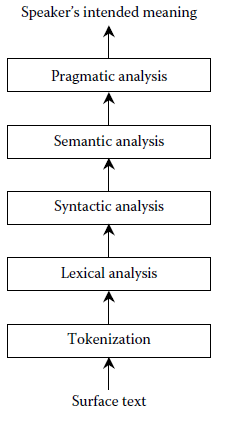
\includegraphics[width=7cm]{pictures/Analyseschritte.png}
\caption{Analyseschritte im klassischen NLP}
\label{fig:STEPS}
\end{wrapfigure} Zur Vorbereitung des Textes auf die weiteren Analyseschritte werden fundamentale Textbausteine, also Wörtern und Sätzen identifiziert. In segmentierten Sprachen wie dem Englischen, wird das \textit{White-Space-Zeichen} zum separieren der einzelnen Worte genutzt. Komplexe Probleme in diesem Zusammenhang sind beispielsweise die richtige Interpretation der Rolle eines Punktes (Satzende, Abkürzung oder Nummerntrennzeichen), der Umgang mit Mehrwortbenennungen oder die Normalisierung des Textes (Vereinheitlichung von unterschiedlicher Schreibweisen eines Wortes).  Hierbei ist die Aussagekraft des Wort- oder Satzkontextes nicht zu unterschätzen. Für die Implementierung der Tokenization existieren zahlreiche regelbasierte Ansätze.\par
Bei der lexikalischen Analyse wird der Text auf Ebene des einzelnen Wortes untersucht. Ein Wort bezeichnet hierbei eine Sammlung von Zeichenfolgen, die zu einem Lemma (Grundform) gehören. Im Rahmen der lexikalischen Analyse wird also einer Zeichenfolge (z.B. schreibt) ein Lemma mit Angaben zur Flexion (z.B. schreiben, 3. Person Singular Präsens) zugeordnet. Außerdem wird die Wortart (\textit{Part-Of Speech}) bestimmt. Im Vergleich zu anderen Sprachen, in denen durch Flexion zahlreiche komplexe Wortformen entstehen, ist diese Aufgabe im Englischen vergleichsweise einfach. Es stehen außerdem umfangreiche lexikale Ressourcen wie zum Beispiel das \textit{Princeton WordNet} für die lexikalische Analyse zur Verfügung. Andererseits entstehen hier erhebliche Schwierigkeiten bei der Identifizierung von Wortarten.\par
Im Rahmen der syntaktische Analyse wird die Struktur eines Satzes analysiert. Zunächst wird die Satzart bestimmt. Den einzelnen Satzbausteinen wird dann ihre grammatikalische Funktion im Satz zugeordnet. Zusätzlich werden erste Ab\-häng\-ig\-keit\-en identifiziert. Der eingesetzte \textit{PCFG-Parser} ist im Idealfall effizient, robust und kann bei Mehrdeutigkeit die wahrscheinlichste Interpretation vorschlagen. PCFG steht für \textit{Probabilistic Context-Free-Grammar.}\par
Ziel der semantischen Analyse ist es, die Bedeutung des Textes zu erfassen. Der originale Text wird hierfür in eine Metasprache übersetzt. Basis hierfür ist die zuvor analysierte syntaktische Struktur der einzelnen Wörter und Sätze. Einige große Problem der semantischen Analyse sind der Umgang mit Mehrdeutigkeit, bildlicher Sprache und Ausdrücken, die aus mehreren Worten zusammengesetzt werden. Der Text wird deshalb in diesem Schritt um verschiedene Wortbedeutung mehrdeutiger Wörter, Wissensdomäne (\textit{Hyperonym}), und Nomen-Pronomen Abhängigkeiten ergänzt (\textit{Coreference Resolution}). Alle extrahierten Informationen werden abschließend in einem \textit{World Model} zusammengetragen, das beispielsweise in einer objektorientierten Datenstruktur realisiert werden kann.\par
Den abschließenden Schritt bildet die pragmatische Analyse. Hier wird entschieden, welche Reaktion aus den gewonnenen Informationen des World Modells abgeleitet werden soll. In der Regel wird ein weiterer Algorithmus mit Parametern versorgt und gestartet. Dieser beantwortet dann entweder eine Eingangsfrage, fasst den Text zusammen oder erstellt eine graphische Repräsenation des Textes wie beispielsweise ein Petri-Netz. Dieser Schritt wird im Rahmen dieser Seminararbeit jedoch nicht betrachtet.

Um einen gegebenen Text mit den genannten Annotationen anreichern zu können, sind spezielle Ressourcen und Tools nötig. Diese werden in Kapitel 3 ausführlich vorgestellt.







\section{Text2Process}

Bei Friedrichs Masterarbeit im intro quellen anschauen.  

World Model nach Buch "Natural Language Processing"




\chapter{NLP Tools}
\section{Stanford CoreNLP}
\label{sec:stanfordparser}

Die Stanford \ac{NLP} Group, ein Team aus Software- und Linguistik Experten, entwickelt quelloffene Software zur Anwendung von \ac{NLP}. Resultat dieser Entwicklung ist eine Menge von Programmen, die jeweils eigenständige \ac{NLP} Probleme lösen und als Software mit eigener Distribution verfügbar sind (\cite[vgl.][1 ff.]{STANFORDNLPTEAM}).  Darunter befindet sich der Stanford Parser. Dieser ist, neben anderen Modulen, aber auch Bestandteil der Stanford CoreNLP Suite, einer seit 2010 offen verfügbaren, vereinigten Distribution der verschiedenen \ac{NLP} Komponenten mit einheitlicher Schnittstelle (\cite[vgl.][1 ff.]{STANFORDNLP}). Das grundlegende Prinzip des Stanford CoreNLPs besteht darin, den zu analysierenden Text in einzelne Elemente, also etwa Worte, zu zerlegen und diese mit Meta-Annotationen verschiedener funktionaler Komponenten zu versehen.\par
Dieses Kapitel soll eine Auswahl derartiger, einzelner Komponenten und ihre Funktionsweise grundlegend erläutern. Zu diesem Zweck wird bei einigen dieser Erläuterungen eine Analyse-Visualisierung folgenden Minimalbeispiels verwendet:
\begin{quote}
"'The student writes his paper at the DHBW. After he is finished, he hands it in."'
\end{quote} Diese Visualisierung wird jeweils anhand eines Web-Tools der Stanford \ac{NLP} Group vorgenommen.\footnote{Erreichbar unter: http://nlp.stanford.edu:8080/corenlp/} Weiterhin soll die Verwendung des Core NLP Toolkits mit Java thematisiert werden. Außerdem sei an dieser Stelle angemerkt, dass der von im State-Of-The-Art Ansatz verwendete Stanford Parser lediglich über die beiden in Abschnitt \ref{subsec:pos} und \ref{subsec:parser} erläuterten Funktionen verfügt.

\subsection{Part-of-Speech}
\label{subsec:pos}

\begin{wrapfigure}{r}{7cm}
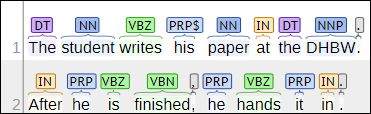
\includegraphics[width=7cm]{pictures/POS.png}
\caption{Visualisierung der POS am Beispiel}
\label{fig:POS}
\end{wrapfigure}

Als \ac{POS} wird die Art eines Wortes bezeichnet. Ein Wort kann beispielsweise ein Nomen, Verb oder Adjektiv sein. Das Stanford CoreNLP über eine Funktionalität, die \ac{POS} Annotationen zu den einzelnen Worten des analysierten Texts hinzufügt.\par
Zu diesem Zweck werden vorhergehende und folgende Wörter im jeweiligen Satz betrachtet. Realisiert wird diese Funktionalität über ein Dependency-Network (\cite[vgl.][1]{POSTAGGER}), das auf die \textit{Penn Treebank} angewandt wird. Dabei handelt es sich um eine Datenbank von syntaktisch analysiertem Text. Abbildung \ref{fig:POS} zeigt das mit POS-Tags versehene Beispiel. Jedes einzelne Wort, wird einer Wortart anhand einer Abkürzung zugeordnet. Beispielsweise steht der dem Wort "'student"' zugeordnete Tag "'NN"' für \textit{Noun}. Der POS-Tagger unterscheidet die 36 verschiedenen Wortarten der Penn Treebank (\cite[vgl.][3]{PENNTREEBANK}), die in Tabelle \ref{table:POSTAGS} vollständig aufgelistet sind.

\subsection{Parser}
\label{subsec:parser}
\begin{wrapfigure}{r}{7cm}
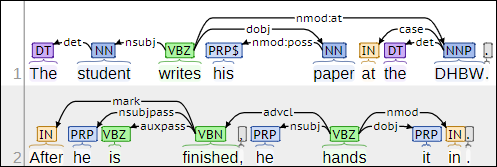
\includegraphics[width=7cm]{pictures/Parser.png}
\caption{Visualisierung der Erweiterten Abhängikeiten am Beispiel}
\label{fig:ENHDEPS}
\end{wrapfigure}
Der Parser des Stanford CoreNLPs baut auf den POS-Tags auf und liefert eine nochmals erweiterte syntaktische Analyse des Textes. Es werden zusätzlich zusammengehörige Phrasen im Satz ermittelt. Dafür werden wiederum zwei unterschiedliche Repräsentationen unterstützt (\cite[vgl.][4]{STANFORDNLP}). Die Analyse kann zum einen durch Abhängigkeiten, zum anderen durch den Aufbau wiedergegeben werden. Abhängigkeiten eines bestimmten Typs werden zwischen zwei Worten gebildet. Die Notation der Analyse nach dem Aufbau erfolgt hingegen anhand einer Baumstruktur. Der Text wird in Phrasen-Typen eingeteilt und die einzelnen Worte diesen zugeordnet.\par Es existieren verschiedene Implementierungsstrategien für den Stanford Parser. Im Stanford CoreNLP wird ein Ansatz anhand eines Neuronalen Netzes verfolgt, der entsprechend auf Wahrscheinlichkeiten basiert. Dieser zeichnet sich vor Allem durch die Realisierung performanter Ausführungszeiten bei einer präzisen Vorhersagegenauigkeit aus (\cite[vgl.][8]{DEPPARSER}).\par
Abbildung \ref{fig:ENHDEPS} zeigt die Syntaktische Analyse anhand der Abhängigkeiten innerhalb der beiden Beispielsätze. So existiert etwa eine Abhängigkeit des Typs det (determiner) vom Wort "'student"' zum Wort "'the"'. Die Schlussfolgerung ist, dass diese beiden Worte eine inhaltliche Phrase bilden.

\subsection{Named-Entity-Recognition}
\label{subsec:ner}
\begin{wrapfigure}{r}{7cm}
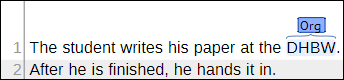
\includegraphics[width=7cm]{pictures/NER.png}
\caption{Visualisierung der NER am Beispiel}
\label{fig:NER}
\end{wrapfigure}
Ein Bestandteil natürlicher Sprache ist die Erwähnung von Eigennamen etwa bestimmter Orte, Personen oder auch Organisationen. Daher verfügt das Stanford CoreNLP über die \ac{NER}. Mit Hilfe dieser Funktionalität können derartige Wörter erkannt und in Bezug auf die Entität, welche sie bezeichnen,  klassifiziert werden. Zu diesem Zweck existieren die vier Kategorien person(PER), location(LOC), organization(ORG) und miscellaneous(MISC) (\cite[vgl.][4]{STANFORDNER}).\par
Beispielsweise könnte ein Wort mit der Annotation "'ORG"' versehen werden, was darauf hinweist, dass es sich dabei um den Namen einer Organisation handelt. So zeigt Abbildung \ref{fig:NER}, dass die Bezeichnung "'DHBW"' im Beispielsatz von der \ac{NER} als Organisation erkannt wird.\par
Zur Implementierung dieses Features wurde eine lexikalische Datenbasis verwendet, weswegen letztlich nicht alle Namen als solche erkannt werden können. Werden bestimmte, mit der \ac{NER} nicht klassifizierbare Namen im Text erwartet, können diese auch regelbasiert anhand eines frei definierbaren Regulären Ausdrucks identifiziert werden (REGEXNER).

\subsection{Coreference Resolution}
\label{subsec:coref}
\begin{wrapfigure}{r}{7cm}
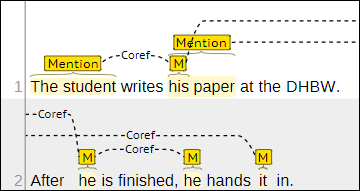
\includegraphics[width=7cm]{pictures/coref.png}
\caption{Visualisierung der Coreference Resolution am Beispiel}
\label{fig:COREF}
\end{wrapfigure}
Ein Text in natürlicher Sprache bezieht sich auf Entitäten nicht nur anhand deren eigentlicher Bezeichnung. In der Regel werden diese Bezeichnungen in derartigen Bezügen auch durch Pronomina o.Ä. ersetzt. Dies kann insbesondere auch satzübergreifend geschehen. Das Stanford CoreNLP ermöglicht über die Coreference Resolution eine Auflösung der Beziehungen zwischen den bezeichneten Entitäten und ihren jeweiligen substitutiven Elementen.\par
Abbildung \ref{fig:COREF} zeigt die Bezüge der Pronomina zu ihren jeweiligen Entitäten über beide Sätze des Beispiels hinweg. 

\subsection{Sentiment Analysis}
\label{subsec:sentiment}
Neben reinem Inhalt verfügt ein Satz in natürlicher Sprache auch über eine Stimmung. Diese äußert sich vorrangig anhand der Auswahl der Worte und deren Konnotation. Das Stanford CoreNLP bietet daher die Sentiment Analysis. Hiermit können Sätze bezüglich ihrer Stimmung als "'negativ"', "'neutral"' oder "'positiv"' annotiert werden.\par
Umgesetzt wird diese Funktionalität unter Anwendung eines rekursiven Neuronalen Netzes, also eines Deep Learning Algorithmus. Zum Training des Netzes wurde die "'Stanford Sentiment Treebank"' verwendet,eine Sammlung von Begriffen versehen mit der jeweiligen Konnotation (\cite[vgl.][1]{SOCHERSENTIMENT}).

\subsection{Java API}
\label{subsec:corenlpjava}
Alle Funktionen des Stanford CoreNLP können unter einem Einheitlichen \ac{API} adressiert werden, welches ursprünglich für die Verwendung unter Java konzipiert wurde. Jedoch existieren auch Implementierungen für andere Sprachen, wie etwa Python, Ruby oder Scala (\cite[vgl.][3]{STANFORDNLP}). Es soll weiterhin die grundlegende Funktionsweise dieser \ac{API} erläutert werden.\par
Die Basis dafür bildet ein Annotation-Objekt, welches reinen Text als Eingabe akzeptiert und nach Ausführung einen annotierten Text ausgibt. Ein mögliches Ausgabeformat für den Annotierten Text ist unter anderem XML. Die funktionalen Module des Stanford CoreNLP, wovon die meisten in diesem Kapitel bereits erkäutert wurden, werden über Annotater repräsentiert. Diese werden sequentiell auf den Text angewendet und fügen Annotationen hinzu. Im Konstruktor des Annotation-Objekts können die gewünschten Annotater über einen String spezifiziert werden (\cite[vgl.][1]{STANFORDNLP}).\par
Weiterhin besteht die Möglichkeit eigene Logik anhand eigener Annotator auszuführen. Hierzu muss ein Interface implementiert werden und der Name der Klasse angegeben. Die Instanzierung erfolgt wie bei den Standard Klassen durch den String des Annotation-Konstruktors über class-reflection (\cite[vgl.][4]{STANFORDNLP}).

\subsection{Weitere Standard NLP-Tookits}

Neben dem Stanford CoreNLP gibt es noch zwei weitere weit verbreitete Standards. Das \ac{NLTK} ist eine Sammlung von Programmmodulen zur Verarbeitung von natürlicher Sprache. Ebenso wie beim Stanford CoreNLP handelt es sich um einen Standard Bibliothek, die grundlegende \ac{NLP} Aufgaben abdeckt. Das \ac{NLTK} steht unter der \textit{GLP Open Source Licence} und wurde für die Programmiersprache Pyhon entwickelt. Es greift auf diverse lexikalische Ressourcen wie WordNet, FrameNet aber auch Wikipedia zurück. Das \ac{NLTK} verfügt im Gegensatz zum Stanford CoreNLP über einfach handhabbare Visualisierungsmodule. Das StanfordCoreNLP kann zwar in Python, das NLTK aber nicht in Java verwendet werden.
\par
Eine weitere Alternative stelle das Apache Projekt OpenNLTK dar. Die Java-Bibliothek ist Machine Learning basiert und erfüllt ebenfalls die gängigen NLP Aufgaben.


%\section{NLTK}

Das \ac{NLTK} ist eine Sammlung von Programmmodulen zur Verarbeitung von natürlicher Sprache. Ebenso wie beim Stanford CoreNLP handelt es sich um einen Standard Bibliothek, die grundlegende \ac{NLP} Aufgaben abdeckt. Das \ac{NLTK} steht unter der GLP open source licence und wurde für die Programmiersprache Pyhon entwickelt. Es greift auf diverse lexikalische Ressourcen wie WordNet, FrameNet aber auch Wikipedia zurück. Das \ac{NLTK} verfügt im Gegensatz zum Stanford CoreNLP über einfach handhabbare Visualisierungsmodule.

Notizen zu Standard NLP Toolkits:
 
 - NLTK kann nicht in java, coreNLP aber in Python genutzt werden
 - Weiteres Open-Source Standard Toolkit: OpenNLTK

\section{Wordnet}


\subsection{Ontologien im NLP}

Bei der zwischenmenschlichen Kommunikation werden Informationen in codierter Form über das Medium der Sprache übertragen. Für den Erfolg des Informationstausches ist die richtige Decodierung der abstrakten Spracheinformationen, das heißt die richtige Verknüpfung eines Wortes mit dessen Bedeutung, entscheidend. 
\begin{quote} \textit{"`In order to effectively exchange information, agents need to share a lexicon of words as well as to access the world model(s) underlying the lexicon."'} (\cite[vgl.][1]{OLTRAMANI})\end{quote} 
Die Kommunikationspartner müssen sowohl über denselben Wortschatz als auch über ein gemeinsames Weltverständnis (engl. \textit{world model}) verfügen. Dies gilt auch für die Mensch-Maschine Kommunikation. Ein World Model kann beispielsweise mittels einer Ontologie in maschinenlesbarer Form abgebildet werden. Eine Ontologie ist in der Informatik definiert als System von Informationen mit logischen Relationen (\cite[vgl.][1]{DUDEN}). Eingeführt wurde der Begriff in de 1970er Jahren auf dem Forschungsgebiet der künstlichen Intelligenz zur Modellierung von Wissen. Ziel von digitalen Ontolgien ist es, Wissensdomänen in maschinenlesbarer Form verfügbar zu machen (\cite[vgl.][7]{TACKE}). Somit sind Ontologien eine zentrale Komponente in Wissenssystemen. 
\par
Das \textit{Princeton WordNet} ist eine solche Ontologie, also eine als semantisches Netz organisierte, lexikalische Ressource. Die Entwicklung von WordNet begann bereits 1985 and der Universität Princeton. 1993 wurde die erste Version veröffentlicht. Die aktuelle Version, das \textit{WordNet 3.0}, enthält etwa 155.000 manuell verfasste Einträge in englischer Sprache. (\cite[vgl.][1]{PRINCETON})
\par
Die aktuelle Version folgt außerdem den Linked Open Data Principles, und somit auch den Grundsätzen des Semantic Web. 
\par
\textit{„Linked Open Data (LOD) is Linked Data which is released under an open licence, which does not impede its reuse for free.“} (\cite[vgl.][1]{BERNERS_LEE}). 
\par
Die freie Verfügbarkeit und die Linked-Data-Struktur haben maßgeblich zur weiten Verbreitung von WordNet beigetragen. Als Metadatenformat in Wordnet wurde die weit verbreitete, standardisierte \textit{Web Ontology Language} eingesetzt. Im \ac{NLP} wird auf WordNet für die Erstellung der semantischen Annotationen benötigt. Es dient als essentielle Ressource für überwacht lernende Algorithmen.
\par

\subsection{Aufbau und Struktur}

Die Basiseinheit in WordNet ist das Wort in seiner Grundform (Lemma). In WordNet werden Wörter mit gleicher oder nahezu identischer Bedeutung in Synsets gruppiert. Der Begriff ist ein Neologismus aus \textit{synonym} (dt. Synonym) und \textit{set} (dt. Menge, Zusammenstellung). Die Synsets werden über Kanten verknüpft, die bestimmte semantische Relationen repräsentieren. So entsteht ein gerichteter azyklischer Graph (\cite[vgl.][12]{OLTRAMANI}), der dem Aufbau des neuronalen Netzes im menschlichen Gehirn ähnelt.Grundsätzlich setzt sich WordNet aus vier Datenbanken für die jeweiligen Wortarten Nomen, Verben, Adjektive und Adverben zusammen. Jede dieser Datenbanken beinhaltet miteinander verknüpfte Synsets. Hierbei wird jeweils auch die Arte der Verknüpfung bzw. der semantischen Relation angegeben. Abhängig von der Wortart sind verschiedene Arten von Relationen möglich. Tabelle \ref{table:table2} zeigt die Relationen von Nomen und Verben in WordNet geordnet nach Häufigkeit.
\par
\begin{table}[h!]
  \centering
  \begin{tabular}{ccccc} %Hier muss für jede Spalte ein c hin -> Dump wegen mismatch von definierter und auftretender Spaltenanzahl
    \toprule
     Rang & Relationen der Nomen & Anteil  & Relationen der Verben & Anteil \\
    \midrule
    1 & Hyponyme/Hypernyme: & 45.5\% & Abgeleitete Form:    & 55.4\% \\
    2 & Abgeleitete Form:   & 22.4\% & Troponyme/Hypernyme: & 31.7\% \\
    3 & Meronyme/Holonymy:  & 13.3\% & Verbgruppe:          & 4.2\%  \\
    4 & Wissensgebiet:      & 9.1\%  & Wissensgebiet:       & 3.0\%  \\
    5 & Typ/Instanz: 		& 5.1\%  & Antonymy:			& 2.6\%  \\
    6 & Pertainyme: 		& 2.9\%  & Siehe auch: 		    & 1.4\%  \\
    7 & Antonyme: 			& 1.3\% & Folgebeziehung: 	    & 1.0\%  \\
	8 & Attribut: 			& 0.4\%  & Ursache: 			& 0.5\%  \\
	9 & Partizip: 	        & 0.2\%  & -     	            & -  	 \\
	\bottomrule
  \end{tabular}
  \caption{Relationen in WordNet (\cite[vgl.][9]{MAZIARZ})}
  \label{table:table2}
\end{table}
\par

Der bei Nomen am häufigsten auftretende Beziehungstyp ist das Hyponym/Hypernym. Diese Beziehung strukturiert die Synsets hierarchisch in übergordnete Elter-Synsets (Hypernym) und untergeordnete Kind-Synsets (Hyponym). Es handelt sich also um eine IS-A-Beziehung. Das äquivalent zu Hyponymen in der Kategorie Verben wird als Troponym bezeichnet. Abgleitete Formen verbinden Synsets über Wortarten-Grenzen hinweg. Beispielsweise ist das Verb \textit{run} mit dem Nomen \textit{run} über die Beziehung der abgeleiteten Form verbunden. Ein weiterer häufiger Beziehungstyp sind Meronyme- und Holonyme-Beziehungen. Sie stellen die Part-Of-Beziehung (Meronym) und deren Gegenstück dar.

\par
\subsection{Word Sense Disambiguation}

Die meisten Worte einer Sprache haben mehrere Bedeutungen. Die richtige Wortbedeutung ergibt sich folglich erst aus dem Kontext der Wortverwendung. Um die Wortbedeutung maschinell zu erfassen, sind ein \textit{Sense Inventory} und ein klassifizierender Algorithmus notwendig. 
\begin{figure}[h]
\begin{center}
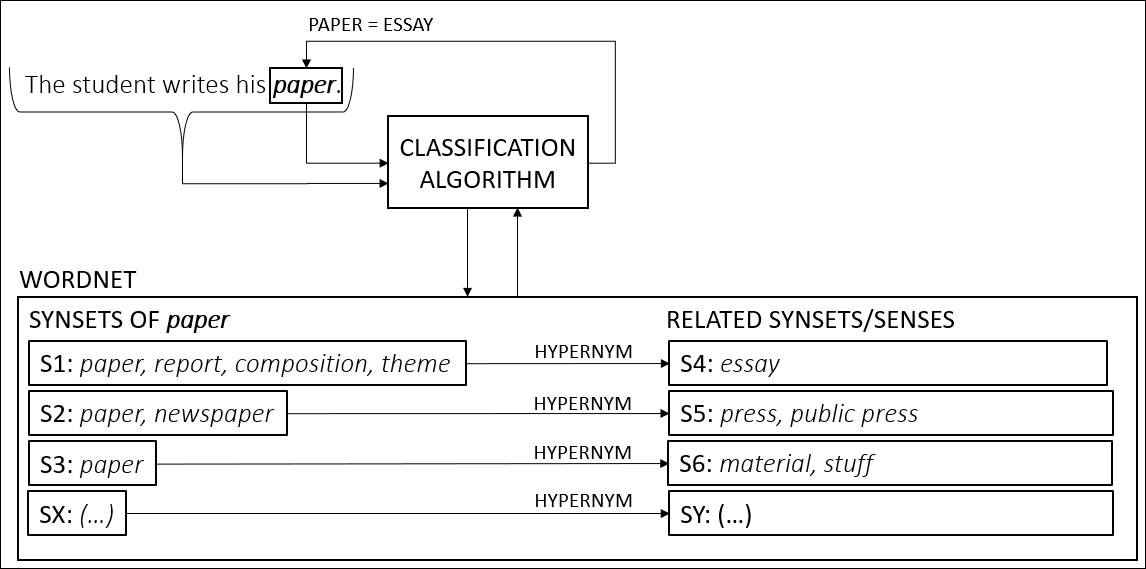
\includegraphics[keepaspectratio=true, width=\textwidth]{pictures/WSD.png}
\caption{WSD Klassifikation mit WordNet (eigene Darstellung)}
\label{fig:WSD}
\end{center}
\end{figure}
Bei einem solchen Sense Inventory handelt es sich um eine Informationsquelle, in der die verschiedenen Wortbedeutungen einsehbar sind. WordNet kann diese Rolle übernehmen. Ein mehrdeutiges Wort ist in WordNet Mitglied in verschiedenen Synsets, aus deren hypernymen Synsets sich dann die verschiedenen Wortbedeutungen ableiten lassen. Abbildung \ref{fig:WSD} zeigt einen Beispielsatz, indem die Bedeutung des englischen Wortes \textit{paper} ermittelt werden soll.
\par 
Der Klassifikationsalogrithmus, hier als Blackbox dargestellt, nutzt die hierarchische Struktur von WordNet um die verschiedenen Bedeutungen nachzuschlagen. Daraufhin wählt er die wahrscheinlichste Bedeutung im Satzzusammenhang aus. In diesem Fall wählt er korrekt die Bedeutung \textit{essay} aus.
\par
Somit ist Word Sense Disambiguation nichts anderes als ein Klassifikationsproblem, das basierend auf gewissen Eingabeparametern eine Einordnung vornimmt. Prinzipiell kann jeder generische, maschinell lernende Klassifikationsalgorithmus zur Lösung herangezogen werden (\cite[vgl.][326]{YAROWSKY}). Als am verlässlichsten stellen jedoch Kombinationen verschiedener Ranking-Algorithem heraus. Die geringe Menge an verfügbaren Trainingsdaten stellt hierbei jedoch immernoch ein Problem dar.


\subsection{Java APIs}

Um WordNet direkt in eigene Softwareprojekte einbinden zu können, stehen allein für die Programmiersprache Java zwölf verschiedenen Bibliotheken zu Verfügung. Bei der Wahl einer geeigneten Bibliothek hängt von verschiedenen Faktoren ab. Im Vergleich schneidet das \textit{\ac{JWI}} für den allgemeinen Anwendungsfall am besten ab (\cite[vgl.][2]{FINLAYSON}). Auch gegenüber der weit verbreiteten \textit{\ac{JWNL}} bietet es nach Finlayson die folgenden Vorteile:

\begin{itemize} 
\item Vollumfänglicher Zugriff auf alle WordNet Ressourcen
\item Arbeitet direkt mit den WordNet-Files (keine Modifizierung notwendig)
\item Dateibasierte und In-Memory-basierte Implementierungsmöglichkeiten
\item Anzahl der instanziierten Dictionaries kann beliebig groß gewählt werden
\item Sehr hohe Performanz, speicherschonend und unabhängig von anderen Systemen
\item Keine \textit{config-Datei} benötigt 
\item Ausführliche Dokumentation, aktiver Support und kontinuierliche Weiterentwicklung
\end{itemize}

Neben der direkten Einbindung von Wordnet über eine Java API, wird Wordnet auch von Standard-Software-Toolkits wie dem Standford CoreNLP oder dem NLTK als Informationsquelle genutzt.
\section{FrameNet}

\subsection{Semantische Frames}

FrameNet ist eine lexikalische Ressource, die in der Universität Berkeley entwickelt wurde und  auf der sprachwissenschaftlichen Theorie der Frame-Semantik nach Charles J. Fillmore basiert (\cite[vgl.][1]{NLTKPROJEKT}).
\par
Um ein Wort oder eine abstrakte Idee begreifen zu können, aktiviert das menschliche Gehirn einen Deutungsrahmen (engl. \textit{frame}). Der Inhalt dieses Frames leitet sich aus dem bestehenden Wissens- und Erfahrungsschatz der jeweiligen Person ab (\cite[vgl.][28]{WEHLING}). Bei dem Wort \textit{tanzen} assoziiert der Leser in der Regel direkt in Verbindung stehende Ideen wie Musik, Choreografie und sich bewegende Menschen. Ein Frame beinhaltet folglich ein ganzes Bündel an Informationen.
\par
Auslöser für die Aktivierung eines Frames sind \textit{Lexical Units}. Hierbei handelt es sich um Wort-Sinnpaare, also um ein Wort und ganz konkretes Verständnis dieses Wortes (\cite[vgl.][1]{NLTKPROJEKT}). Beispielsweise kann das Wort \textit{treffen}, im Sinne von \textit{begegnen}, den Frame \textit{Begegnung} aktivieren, mit dem in der Regel zwei Personen, Händeschütteln oder Grußworte assoziiert werden. \textit{Treffen} im Sinne von \textit{ein Ziel treffen} erweckt ganz andere Erinnerungen und somit einen anderen Frame. Bei der aktivierenden Lexical Unit muss es sich jedoch nicht zwangsläufig um ein einzelnes Wort halten. Auch Ausdrücke mit mehreren Wörtern können eine Lexical Unit bilden.
\par
Als Valenz wird die Fähigkeit eines Wortes bezeichnet, andere Wörter an sich zu binden. Ein Valenzmuster ist somit eine syntaktische Schablone für den üblichen Gebrauch eines Wortes. Wird ein Wort in einem Satz ohne Berücksichtung der in der jeweiligen Sprache üblichen Valenzmuster eingebaut, klingt das Resultat falsch oder ungewohnt.
\par
Die mit einem Frame assoziierten Vokabeln werden als \textit{Frame Elemente} bezeichnet. Über sie steht der Frame in Verbindung mit anderen Frames. 

\subsection{Aufbau und Struktur}

Ähnlich wie WordNet, ist FrameNet ebenfalls als azyklischer Graph strukturiert. Die Knoten bilden jedoch nicht Synsets, sondern Frames under deren Frame Elemente. Die Beziehungen zwischen den Frames sind die Kanten. FrameNet ist weniger granular als WordNet in der Unterscheidung von Wortbedeutungen. Ähnlich wie in WordNet existieren auch in FrameNet verschiedene Beziehungstypen.
\par
Die Vererbungsrelation \textit{Inheritance} stellt eine IS-A-Relation dar. Jedes Frame Element im Eltern-Frame ist mit koresspondierenden Frame-Elementen im Kind-Frame verbunden. Ein \textit{Subframe} stellt ein Subevent zu einem komplexeren oder abstrakten Eltern-Frame dar. Der 
\textit{Using}-Beziehungstyp nutzt den Eltern-Frame als Hintergrund. Nicht alle Eltern-Frame-Elemente müssen jedoch mit Kinde-Frame-Elementen verbunden sein. Darüber hinaus gibt es noch weitere, seltener auftretende Beziehungstypen.


\subsection{Semantic Role Labeling}

Ein Hauptanwendungsgebiet für FrameNet ist das \ac{SRL}. Hierbei wird einem Satzglied, in der Linguistik auch als \textit{Argument} bezeichnet, eine abstrakte Rolle zugewiesen. Die semantische Satzaussage, das \textit{Prädikat}, ergibt sich dann aus der Summe der Argumente. Aus diesem flachen semantischen Repräsentationslevel können dann Informationen extrahiert werden.
\par
Ein Problem des \ac{SRL} ist die einheitliche Definition von Rollen. Abhängig vom Abstraktonsgrad können konkrete Rollendefinitionen (\textit{Deep Roles}) oder abstrakte Rollendefinitionen (\textit{Thematic Roles}) verwendet werden. Typische Beispiele für thematische Rollen sind beispielsweise (\cite[vgl.][379]{JURAFSKY}):
\begin{itemize}
\item AGENT: Verursache eines Ereignisses.
\item THEME: Direkt vom Ereignis beeinflusstes Satzglied
\item INSTRUMENT: In einem Ereignis verwendeter Gegenstand
\item GOAL: Ziel eines Objektes in einem Transferevent.
\end{itemize}
Die tatsächlich verwendeten Rollendefinitionen unterschieden sich von Implementierung zu Implementierung.

Die semantischen Rollen stehen nicht zwangsläufig in Beziehung zu der syntaktischen Rolle der Satzglieder. Abbildung  \ref{fig:SEMAFOR1} zeigt den Manager als Subjekt des Satzes. Abbildung \ref{fig:SEMAFOR2} zeigt die E-Mail als Subjekt des Satzes. In beiden Fällen erfüllt der Manager die Rolle des Authors und die E-Mail die Rolle des Textes.
\par
\begin{wrapfigure}{r}{8cm}
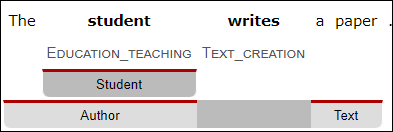
\includegraphics[width=7cm]{pictures/SEMAFOR1.png}
\caption{\ac{SRL} Annotationen: Beispiel 1 (Quelle: http://demo.ark.cs.cmu.edu/parse)}
\label{fig:SEMAFOR1}
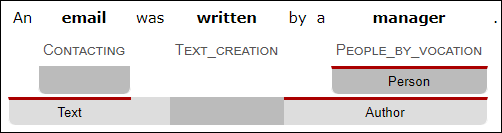
\includegraphics[width=7cm]{pictures/SEMAFOR2.png}
\caption{\ac{SRL} Annotationen: Beispiel 2 (Quelle: http://demo.ark.cs.cmu.edu/parse)}
\label{fig:SEMAFOR2}
\end{wrapfigure}
\par
Eine solche Veränderung der Argumentreihenfolge wird als \textit{Diathesis Alternation} bezeichnet. Die Menge der möglichen Argumentfolgen die zu einem bestimmten Verb gehören werden als \textit{Thematic Grid} oder \textit{Case Frame} bezeichnet. In FrameNet entspricht dies also der Summe der möglichen Valenzmuster. Die zu füllenden Rollen eines Frames in FrameNet entsprechen den Frame Elements (\cite[vgl.][383]{JURAFSKY}).
\par
\ac{SRL} kann automatisch durchgeführt werden. Es existieren einige \ac{SRL} Systeme, die überwachte Machine Learning Algorithmen auf Basis von FrameNet durchführen. Beispiele hierfür sind SEMAFOR, MatePlus und Open-SESAME. Der modernste und performanteste Ansatz ist das Python-basierte System Open-SESAME (\cite[vgl.][8]{SWAYAMDIPTA}), das auch ohne vorausgehendes syntaktisches Parsen State-of-the-Art-Qualität liefert.
Neben FrameNet eignen sich auch andere lexikalische Ressourcen für \ac{SRL}. Auch die Ressourcen PropBank und VerbNet kommen hierfür in Frage.


\chapter{State-Of-The-Art Analyse}
\section{State-Of-The-Art Analyse}

\subsection{Betrachtungsgegenstand}
Der derzeitige State-Of-The-Art im Bereich \ac{T2P} ist das Verfahren von Friedrich aus dem Jahr 2011 (\cite[vgl.][11]{RIEFER}). Im Folgenden wird die von Friedrich erarbeitete Vorgehensweise (\cite[vgl.][11]{FRIEDRICH1} und \cite[vgl.][11]{FRIEDRICH2}) analysiert und Verbesserungsvorschläge erarbeitet.
Die Analyse beschränkt sich auf die Textverarbeitung bishin zur generierung des World Models. Die Konstruktion eines Graphen aus dem World Model ist nicht Teil dieser Arbeit.
\par
Zunächst wird im Folgenden kurz auf den konkreten Aufbau des World Models nach Friedrich eingegangen. Anschließend folgt die Analyse der Vorgehensweise. Gemäß der durch Friedrich vorgegebenen Gliederung wird zunächst die Textverarbeitung auf Satz-Ebene und dann die Textverarbeitung auf Text-Ebene analysiert. Abschließend werden bekannte Problemfelder zusammengetragen und Lösungsansätze vorgeschlagen.

\subsection{World Model}
World Model: Actor, Resource, Action, Flow
Enrichment of Worldmodel step by step
(= Ziel)

\subsection{Textverarbeitung auf Satz-Ebene}

Der Eingangstext in natürlicher Sprache wird zunächst in einzelne Wörter und Sätze aufgesplittet. In \ref{fig:SLEVEL} wird dieser Vorgang der \textit{Sentence Decomposition} zugeordnet. Es handelt sich hierbei um eine normale Tokenization, bei der auf die Stanford CoreNLP Funktionen \textit{Stanford TokenizerAnnotator} und \textit{Stanford WordsToSentenceAnnotator} zurückgegriffen wird. Im nächsten Schritt wird der Text mit dem \textit{POSTaggerAnnotator} mit \textit{POS-Tags} versehen und anschließend mit dem PCFG-Parser \textit{ParserAnnotator} die Satzstruktur analysiert. Dies wird durch den Pfeil von StanfordParser zu Subprozess in \ref{fig:SLEVEL} symbolisiert. Auf eine pauschale \textit{Lemmatization} aller Wörter wird an dieser Stelle verzichtet.

\begin{wrapfigure}{r}{13cm}
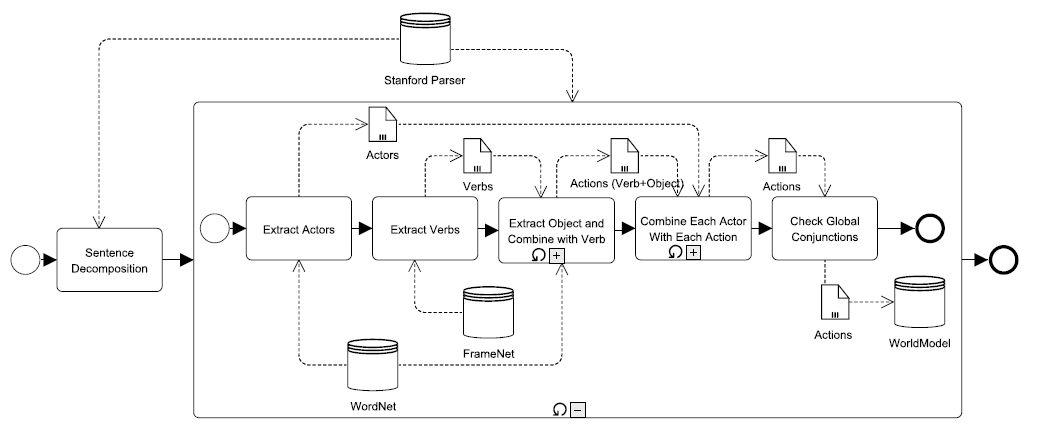
\includegraphics[width=13cm]{pictures/SentenceLevel.png}
\caption{Analyseschema auf Satzebene (\cite[vgl.][5]{FRIEDRICH2})}
\label{fig:SLEVEL}
\end{wrapfigure}

Auf Basis der Annotationen folgt dann das \textit{Phrase Chunking}, der zweite Teil der Sentence Decomposition. Die annotierten Informationen...




Algorithm phrase chunking (problem of complex sentences)
- check if active or passive (Active-passive issue)
- Actors and actions are extracted and filtering (example sentences filtered out with stop word list)
-->SRL Task
- combining each action with each object
- same with actors, action has to be atomic
- all are added to world model

Step 2 Text Level Analysis:
- taking sentence relationships into account
- resolve relative references in text (anaphora relolution algorithm issue 4.1)
- conditional markers (based on 4 lists, AI?)
combine info in different actions (2.2) wich are split over sentences
- dafür: merger candidates with anaphora resolution
- textua links: 3 typen von links forwärts, rückwärts und jumper
- vergleich übe root form
-last step: Flow generation
- bisher nur or, and/or und and


Thesis:
Anaphora resolution:
pronouns, determiners, relative pronouns ok. Problem: Steve Jobs = CEO of Apple

Semantic Role Labelling
Extract Actor, Resource, Actions, Flows

1) Decomposition (Tokenization)
2) Parsing

issue cathegories: Syntactic Leeway, Atomiticity, Relevance, Referencing
--> Classic NLP tasks

\subsection{Textverarbeitung auf Text-Ebene}
\subsection{Problemfelder und Lösungsansätze}





\chapter{Zusammenfassung und Ausblick}
\section{Zusammenfassung und Fazit}
Diese Arbeit befasste sich ausführlich mit der Darstellung und den Anwendungsmöglicheiten von \ac{AI} Tools auf die Prozessmodell Generierung aus Beschreibungen in natürlicher, englischer Sprache. 
Die Betrachtung des State-Of-The-Art Ansatzes hat gezeigt, dass sich mit der Weiterentwicklung der \ac{NLP} betrachteten Tools an manchen Stellen des Verfahrens neue Möglichkeiten ergeben.\par
Folglich wurden die Grundlagen und Tools zum Thema Text-2-WorldModel erläutert sowie der State-Of-The-Art Ansatz analysiert. Das in Kapitel \ref{SUBSEC:ZIEL} formulierte Ziel wurde somit erreicht.

\section{Ausblick}
Letztlich soll auf die Frage eingegangen werden, wie sich der State-Of-The-Art Ansatz verbessern lässt. Als Benchmark könnte hierfür die in   Bei Friedrichs State-Of-The-Art Ansatz handelt es sich um einen regelbasierten Ansatz, der sich auch der Anwendung von Heuristiken bedient. Natürliche Sprache kann nicht vollständig an Regeln festgemacht werden, denn es bleibt immer ein Interpretationsspielraum. Folglich Bedarf es auch für die \ac{T2P} an menschlicher Interpretation. \par
Die Anwendung der Machine Learning Methode supervised learning wird bei ähnlichen Problemen bereits angewendet und verspricht effektive Resultate (\cite[vgl.][2]{BPMML}). Es Bedarf allerdings einer Datenbasis von inputs und outputs.

\addcontentsline{toc}{chapter}{Literaturverzeichnis}
\printbibliography


\appendix     
\part*{Anhang} % Start the appendix part
   
    
\chapter{Anhang} 

\section{POS-Tags}

\begin{longtable}{|l|l|l|}
\caption{Liste aller POS-Tags der Penn Treebank (\cite[vgl.][8]{PENNTREEBANK})}\\
\hline \multicolumn{1}{|c|}{\textbf{ }} & \multicolumn{1}{c|}{\textbf{Tag}} & \multicolumn{1}{c|}{\textbf{Bedeutung}} \\ \hline 
\endfirsthead

\multicolumn{3}{c}%
{{\bfseries \tablename\ \thetable{} -- Weiterführung}} \\
\hline \multicolumn{1}{|c|}{\textbf{ }} & \multicolumn{1}{c|}{\textbf{Tag}} & \multicolumn{1}{c|}{\textbf{Bedeutung}} \\ \hline 
\endhead

\hline \multicolumn{3}{|r|}{{Weiterführung auf nächster Seite}} \\ \hline
\endfoot

\hline \hline
\endlastfoot
 1. & CC & Coordinating conjunction \\
	 2. & CD & Cardinal number\\
	 3. & DT & Determiner \\
	4.&  EX &	Existential there\\
	5.&	FW &	Foreign word\\
	6.&	IN &	Preposition or subordinating conjunction\\
	7.&	JJ &	Adjective\\
	8.&	JJR &	Adjective, comparative\\
	9.&	JJS &	Adjective, superlative\\
	10.& LS &	List item marker\\
	11.& MD &	Modal\\
	12.& NN &	Noun, singular or mass\\
	13.& NNS &	Noun, plural\\
	14.& NNP &	Proper noun, singular\\
	15.& NNPS &	Proper noun, plural\\
	16.& PDT & Predeterminer\\
	17.& POS & Possessive ending\\
	18. & PRP & Personal pronoun \\
	19.& PRP\$ & Possessive pronoun\\
	20.& RB & Adverb\\
	21.& RBR & Adverb, comparative\\
	22.& RBS & Adverb, superlative\\
	23.& RP & Particle\\
	24.& SYM & Symbol\\
	25.& TO & to\\
	26.& UH & Interjection\\
	27.& VB & Verb, base form\\
	28.& VBD & Verb, past tense\\
	29.& VBG & Verb, gerund or present participle\\
	30.& VBN & Verb, past participle\\
	31.& VBP & Verb, non-3rd person singular present\\
	32.& VBZ & Verb, 3rd person singular present\\
	33.& WDT & Wh-determiner\\
	34.& WP & Wh-pronoun\\
	35.& WP\$ & Possessive wh-pronoun\\
	36.& WRB & Wh-adverb	\\

	  \label{table:POSTAGS}
\end{longtable}



\section{Stanford Dependency-Tags}

\begin{longtable}{|l|l|l|}

  \caption{Liste aller DEP-Tags des Stanford Parsers (\cite[vgl.][3 ff.]{STANFORDDEPS})}\\
\hline \multicolumn{1}{|c|}{\textbf{     }} & \multicolumn{1}{c|}{\textbf{Tag}} & \multicolumn{1}{c|}{\textbf{Bedeutung}} \\ \hline 
\endfirsthead

\multicolumn{3}{c}%
{{\bfseries \tablename\ \thetable{} -- Weiterführung}} \\
\hline \multicolumn{1}{|c|}{\textbf{     }} & \multicolumn{1}{c|}{\textbf{Tag}} & \multicolumn{1}{c|}{\textbf{Bedeutung}} \\ \hline 
\endhead

\hline \multicolumn{3}{|r|}{{Weiterführung auf nächster Seite}} \\ \hline
\endfoot

\hline \hline
\endlastfoot
  1. & acomp & adjectival complement \\
2. & advcl & adverbial clause modifier\\
3. & advmod & adverb modifier\\
4. & agent & agent\\
5. & amod & adjectival modifier\\
6. & appos & appositional modifier\\
7. & aux & auxiliary\\
8. & auxpass & passive auxiliary\\
9. & cc & coordination\\
10. & ccomp & clausal complement\\
11. & conj & conjunct\\
12. & cop & copula\\
13. & csubj & clausal subject\\
14. & csubjpass & clausal passive subject\\
15. & dep & dependent\\
16. & det & determiner\\
17. & discourse & discourse element\\
18. & dobj & direct object\\
19. & expl & expletive\\
20. & goeswith & goes with\\
21. & iobj & indirect object\\
22. & mark & marker\\
23. & mwe & multi-word expression\\
24. & neg & negation modifier\\
25. & nn & noun compound modifier\\
26. & npadvmod & noun phrase as adverbial modifier\\
27. & nsubj & nominal subject\\
28. & nsubjpass & passive nominal subject\\
29. & num & numeric modifier\\
30. & number & element of compound number\\
31. & parataxis & parataxis\\
32. & pcomp & prepositional complement\\
33. & pobj & object of a preposition\\
34. & poss & possession modifier\\
35. & possessive & possessive modifier\\
36. & preconj & preconjunct\\
37. & predet & predeterminer\\
38. & prep & prepositional modifier\\
39. & prepc & prepositional clausal modifier\\
40. & prt & phrasal verb particle\\
41. & punct & punctuation\\
42. & quantmod & quantifier phrase modifier\\
43. & rcmod & relative clause modifier\\
44. & ref & referent\\
45. & root & root\\
46. & tmod & temporal modifier\\
47. & vmod & reduced non-finite verbal modifier\\
48. & xcomp & open clausal complement\\
49. & xsubj & controlling subject\\

\end{longtable}

\section{Beigabenverzeichnis}
\begin{enumerate}
	\item Seminararbeit
	\begin{enumerate}
		\item Seminararbeit Text2WorldModel.pdf
	\end{enumerate}

\end{enumerate} 



\end{document}
